\begin{homeworkProblem}
The problem is to find a general solution to:
\[
u_{xx}  + u = 6y
\]
in terms of arbitrary functions; where $u=u(x,t)$.
Here, the general solution is seen to be:
\[
u = A\left( y \right)\sin \left( x \right) + B\left( y \right)\cos \left( x \right) + 6y
\]
where $A(y)$ and $B(y)$ are arbitrary. This general solution can be verified directly:
\[
u_{xx}  + u = \left[ { - A\left( y \right)\sin \left( x \right) - B\left( y \right)\cos \left( x \right)} \right] + \left[ {A\left( y \right)\sin \left( x \right) + B\left( y \right)\cos \left( x \right) + 6y} \right] = 6y
\]
as required.
\end{homeworkProblem}
\begin{homeworkProblem}
The problem is to find a general solution to:
\[
u_{tx}  + u_x  = 1
\]
in terms of arbitrary functions; where $u=u(x,t)$. To begin, one may integrate both sides with respect to $x$:
\[
\int {u_{tx} dx}  + \int {u_x dx}  = \int {1dx}  \Rightarrow u_t  + u = x + f\left( t \right)
\]
for some arbitrary function $f(x)$. At this point, we may solve for $u$ using the method of integration factors:
\[
u = \frac{{\int {\left( {x + f\left( t \right)} \right)e^{\int {1dt} }  + g\left( x \right)} }}
{{e^{\int {1dt} } }} = \left[ {\int {\left( {x + f\left( t \right)} \right)e^t dt + g\left( x \right)} } \right]e^{ - t} 
\]

where $g(x)$ is an arbitrary function. This general solution may be verified directly:
\[
\frac{\partial }
{{\partial t}}\left( {\frac{\partial }
{{\partial x}}\left( {\left[ {\int {\left( {x + f\left( t \right)} \right)e^t dt + g\left( x \right)} } \right]e^{ - t} } \right)} \right) + \frac{\partial }
{{\partial x}}\left( {\left[ {\int {\left( {x + f\left( t \right)} \right)e^t dt + g\left( x \right)} } \right]e^{ - t} } \right)
\]
and since:
\[
\frac{\partial }
{{\partial x}}\left( {\left[ {\int {\left( {x + f\left( t \right)} \right)e^t dt + g\left( x \right)} } \right]e^{ - t} } \right) = \frac{\partial }
{{\partial x}}e^{ - t} \int {xe^t dt}  + \frac{\partial }
{{\partial x}}e^{ - t} \int {f\left( t \right)e^t dt}  + e^{ - t} g'\left( x \right)
\]
\[
 = 1 + g'\left( x \right)e^{ - t} 
\]
we get:
\[
 \Rightarrow u_{tx}  + u_x  = \frac{\partial }
{{\partial t}}\left( {1 + g'\left( x \right)e^{ - t} } \right) + 1 + g'\left( x \right)e^{ - t}  =  - g'\left( x \right)e^{ - t}  + 1 + g'\left( x \right)e^{ - t}  = 1
\]
\[
 \Rightarrow u_{tx}  + u_x  = 1
\]

as required.
\end{homeworkProblem}
\begin{homeworkProblem}
The problem is to show that the general solution $u = u\left( {x,y} \right)$ of $yu_x  - xu_y  = 0$ is given by $
u = \psi \left( {x^2  + y^2 } \right)$, where $\psi$ is an arbitrary function.
First, consider the parameterization:
\[
x = r\cos \left( \theta  \right),y = r\sin \left( \theta  \right)
\]
From this, we see that:
\[
\left. {\begin{array}{*{20}c}
   {x = r\cos \left( \theta  \right)}  \\
   {y = r\sin \left( \theta  \right)}  \\

 \end{array} } \right\} \Rightarrow \left. {\begin{array}{*{20}c}
   {r = \sqrt {x^2  + y^2 } }  \\
   {\theta  = \arctan \left( {\frac{y}
{x}} \right)}  \\

 \end{array} } \right\}
\]
\[
 \Rightarrow \frac{{\partial r}}
{{\partial x}} = \frac{1}
{{2\sqrt {x^2  + y^2 } }} \cdot 2x = \frac{x}
{{\sqrt {x^2  + y^2 } }} = \frac{{r\cos \left( \theta  \right)}}
{r} = \cos \left( \theta  \right)
\]
\[
 \Rightarrow \frac{{\partial r}}
{{\partial y}} = \frac{1}
{{2\sqrt {x^2  + y^2 } }} \cdot 2y = \frac{y}
{{\sqrt {x^2  + y^2 } }} = \frac{{r\sin \left( \theta  \right)}}
{r} = \sin \left( \theta  \right)
\]
\[
 \Rightarrow \frac{{\partial \theta }}
{{\partial x}} =  - \frac{y}
{{\left( {1 + \left( {\frac{y}
{x}} \right)^2 } \right)x^2 }} =  - \frac{y}
{{x^2  + y^2 }} =  - \frac{{\sin \left( \theta  \right)}}
{r}
\]
\[
 \Rightarrow \frac{{\partial \theta }}
{{\partial y}} = \frac{x}
{{x^2  + y^2 }} = \frac{{\cos \left( \theta  \right)}}
{r}
\]
Next, consider an auxiliary function defined by: \[
\upsilon \left( {r,\theta } \right) = u\left( {r\cos \left( \theta  \right),r\sin \left( \theta  \right)} \right)
\]
Writing the given PDE in terms of $\upsilon$ gives:
\[
yu_x  - xu_y  = 0 \Rightarrow r\sin \left( \theta  \right)\left( {\frac{{\partial \upsilon }}
{{\partial r}}\frac{{\partial r}}
{{\partial x}} + \frac{{\partial \upsilon }}
{{\partial \theta }}\frac{{\partial \theta }}
{{\partial x}}} \right) - r\cos \left( \theta  \right)\left( {\frac{{\partial \upsilon }}
{{\partial r}}\frac{{\partial r}}
{{\partial y}} + \frac{{\partial \upsilon }}
{{\partial \theta }}\frac{{\partial \theta }}
{{\partial y}}} \right) = 0
\]
\[
 \Rightarrow r\sin \left( \theta  \right)\cos \left( \theta  \right)\upsilon _r  - \sin ^2 \left( \theta  \right)\upsilon _\theta   - r\sin \left( \theta  \right)\cos \left( \theta  \right)\upsilon _r  - \cos ^2 \left( \theta  \right)\upsilon _\theta   = 0
\]
\[
 \Rightarrow  - \left[ {\sin ^2 \left( \theta  \right) + \cos ^2 \left( \theta  \right)} \right]\upsilon _\theta   = 0 \Rightarrow \upsilon _\theta   = 0 \Rightarrow \upsilon \left( {r,\theta } \right) = f\left( r \right)
\]
where $f(r)$ is an arbitrary function. Since $r = \sqrt {x^2  + y^2 } $, we may conclude the $u$ is an arbitrary function of $\sqrt {x^2  + y^2 } $ (or, equivelantly, an arbitrary function of $x^2  + y^2$):
\[
u\left( {x,y} \right) = \psi \left( {x^2  + y^2  } \right)
\]
as required.
\end{homeworkProblem}

\begin{homeworkProblem}
The problem is to determine the regions in the plane where the equation 
$yu_{xx}  - 2u_{xy}  + xu_{yy}  = 0$ is parabolic, elliptic, or 
hyberbolic. The discriminant is computed to be $\left( { - 2} \right)^2  - 4xy = 4\left( {1 - xy} \right)$. Each case is now considered in turn:
\begin{enumerate}[(a)]
\item (Parabolic): For this case, we must have $4\left( {1 - xy} \right) = 0 \Rightarrow 1 - xy = 0 \Rightarrow y = \frac{1}{x}$. So, $yu_{xx}  - 2u_{xy}  + xu_{yy}  = 0$ is parabolic along the points on $y = \frac{1}{x}$
\item (Elliptic): For this case, we must have $
4\left( {1 - xy} \right) < 0 \Rightarrow xy > 1 \Rightarrow \left\{ {\begin{array}{*{20}c}
   {y < {\raise0.7ex\hbox{$1$} \!\mathord{\left/
 {\vphantom {1 x}}\right.\kern-\nulldelimiterspace}
\!\lower0.7ex\hbox{$x$}}} & {{\text{for }}x < 0}  \\
   {y > {\raise0.7ex\hbox{$1$} \!\mathord{\left/
 {\vphantom {1 x}}\right.\kern-\nulldelimiterspace}
\!\lower0.7ex\hbox{$x$}}} & {{\text{for }}x > 0}  \\

 \end{array} } \right.
$. So, $yu_{xx}  - 2u_{xy}  + xu_{yy}  = 0$ is elliptic in the portion of the plane complimentry to the area between the two curves which comprise $y = \frac{1}{x}$.
\item (Hyperbolic):
For this case, we must have $
4\left( {1 - xy} \right) > 0 \Rightarrow xy < 1 \Rightarrow \left\{ {\begin{array}{*{20}c}
   {y > {\raise0.7ex\hbox{$1$} \!\mathord{\left/
 {\vphantom {1 x}}\right.\kern-\nulldelimiterspace}
\!\lower0.7ex\hbox{$x$}}} & {{\text{for }}x < 0}  \\
   {y < {\raise0.7ex\hbox{$1$} \!\mathord{\left/
 {\vphantom {1 x}}\right.\kern-\nulldelimiterspace}
\!\lower0.7ex\hbox{$x$}}} & {{\text{for }}x > 0}  \\

 \end{array} } \right.
$. So, $yu_{xx}  - 2u_{xy}  + xu_{yy}  = 0$ is hyperbolic in the area of the plane between the two curves which comprise $y = \frac{1}{x}$.

\end{enumerate}
\begin{figurehere}
\centering
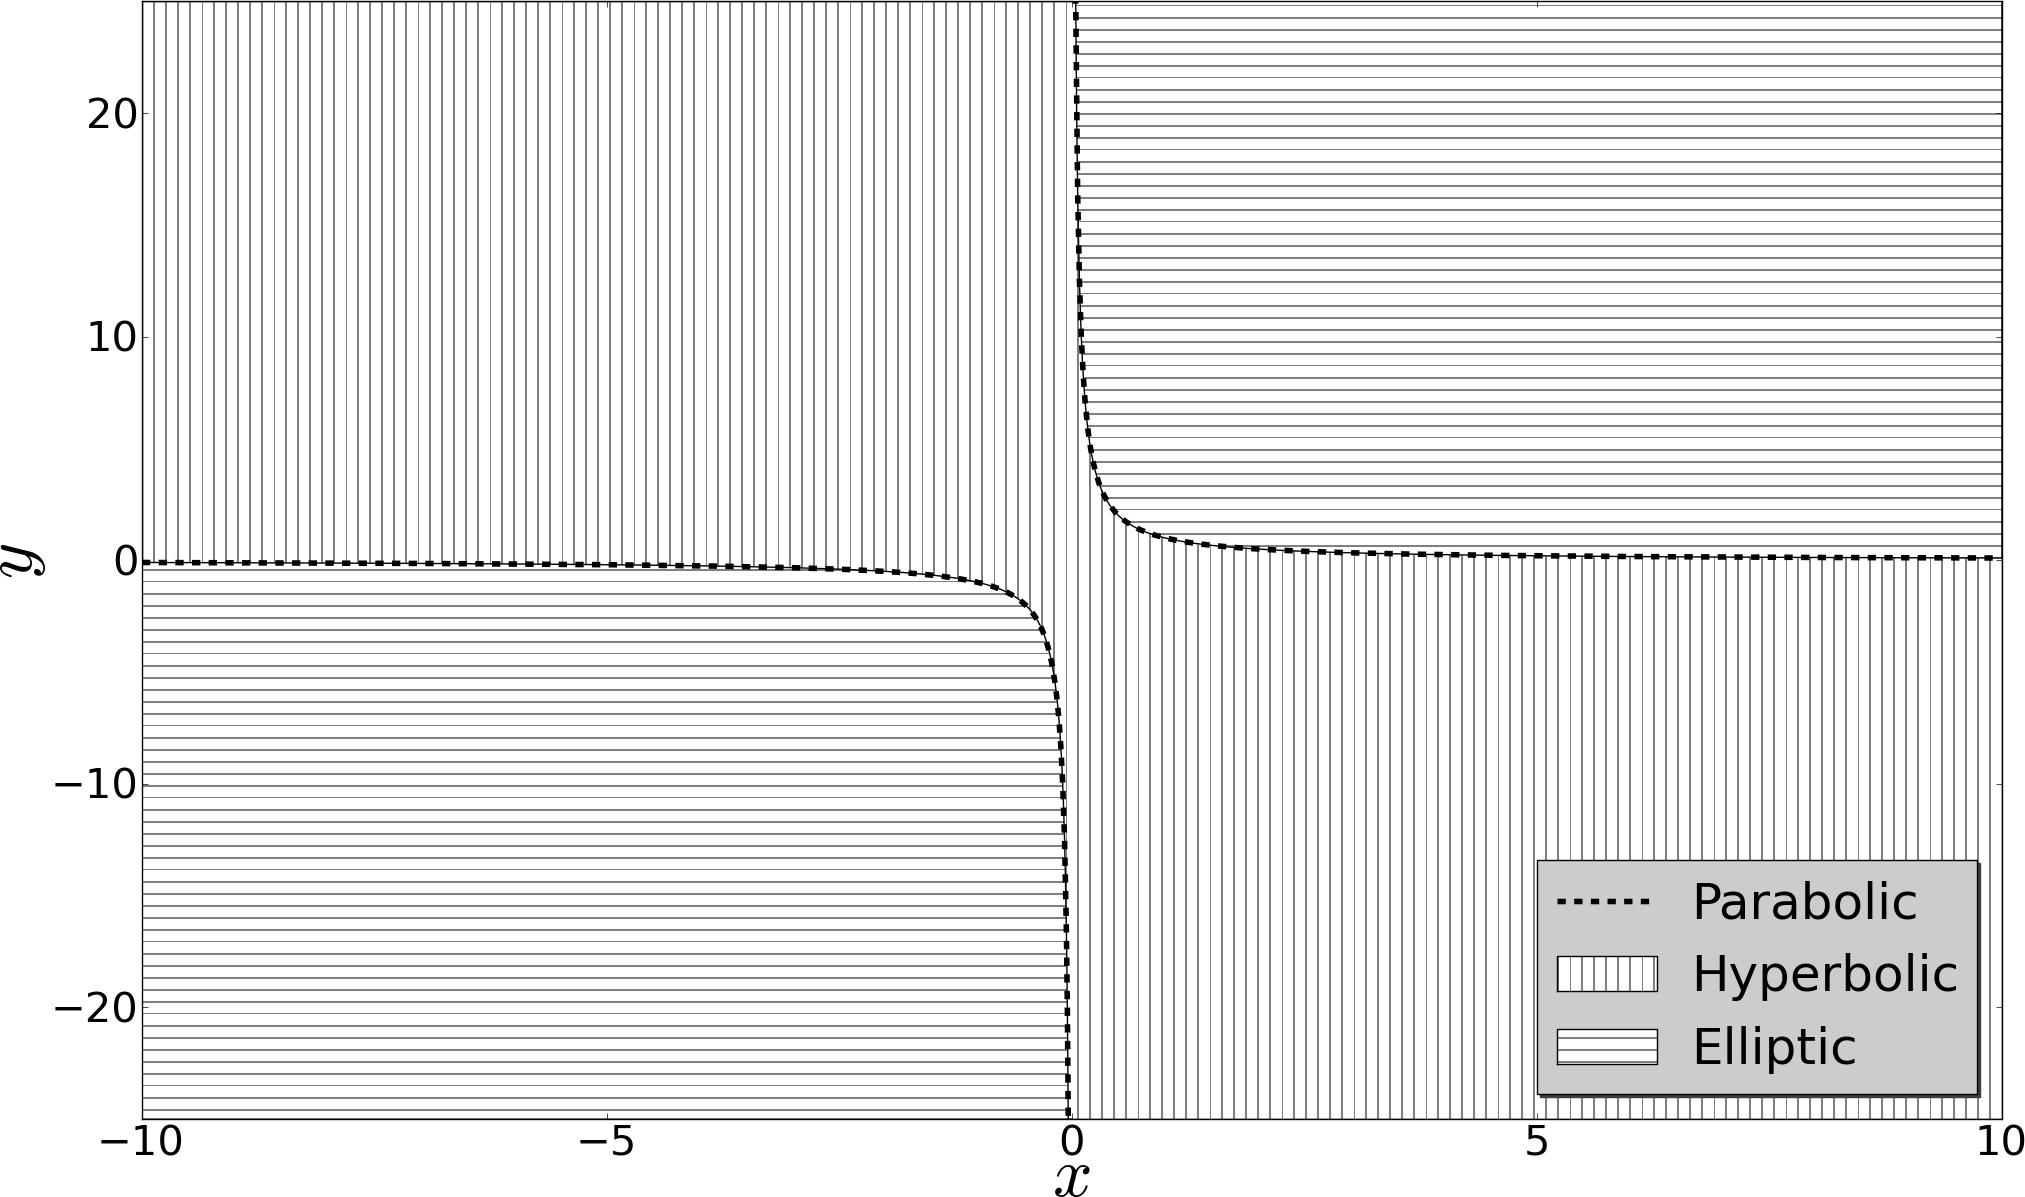
\includegraphics[width=1\columnwidth]{22_1.png}
\caption{(Problem 22) A plot showing where the equation $yu_{xx}  - 2u_{xy}  + xu_{yy}  = 0$ is parabolic, elliptic, and hyberbolic.}
\end{figurehere}
\end{homeworkProblem}

\begin{homeworkProblem}
The problem is to show that the growth-diffusion equation $u_t  = D\Delta u + ru$ can be tranformed into a pure diffusion equation via the transformation $v = ue^{ - rt}$. The definition of the transformation gives:
 \[
v = ue^{ - rt}  \Rightarrow u = ve^{rt} 
\]
and thus:
\[
u_t  = v_t e^{rt}  + vre^{rt} 
\]
Since the Laplacian operator treats $t$ as a constant, we have:
\[
\Delta u = \Delta \left[ {ve^{rt} } \right] = e^{rt} \Delta v
\]
So the original PDE can be written as:
\[
v_t e^{rt}  + vre^{rt}  = \Delta ve^{rt}  + vre^{rt}  \Rightarrow v_t e^{rt}  = e^{rt} \Delta v \Rightarrow v_t  = \Delta v
\]
which is in the form of a pure diffusion equation.
\end{homeworkProblem}

\begin{homeworkProblem}
The problem is to prove the non-optimal Poincar\'{e} inequality:
\[
\left\| u \right\|_2^2  \leqslant \frac{{L^2 }}
{4}\left\| {u_x } \right\|_2 
\]
for all sufficiently smooth functions $u$ satisfying $u(0)=u(L)=0$.
To begin, we know from the fundamental theorem of calculus and the given conditions $u(0)=u(L)=0$ that:
\[u = \int\limits_0^x {{u_x}}  =  - \int\limits_0^L {{u_x}} \]
Using the first part of the above equation, note that:
\[\left| u \right| = \left| {\int\limits_0^x {{u_x}} } \right| \leqslant \int\limits_0^x {\left| {{u_x}} \right|} \]
From the Cauchy-Schwartz inequality $\int\limits_0^L {\left| {fg} \right|}  \leqslant {\left\| f \right\|_2}{\left\| g \right\|_2}$, we have:
\[\int\limits_0^x {\left| {{u_x}} \right|}  \leqslant {\left[ {\int\limits_0^x {{{\left| {{u_x}} \right|}^2}} } \right]^{\frac{1}{2}}}{\left[ {\int\limits_0^x {{{\left| 1 \right|}^2}} } \right]^{\frac{1}{2}}} = {\left[ {\int\limits_0^x {{{\left| {{u_x}} \right|}^2}} } \right]^{\frac{1}{2}}}{x^{\frac{1}{2}}} \leqslant {\left[ {\int\limits_0^L {{{\left| {{u_x}} \right|}^2}} } \right]^{\frac{1}{2}}}{x^{\frac{1}{2}}}\]
and thus:
\[{\left| u \right|^2} \leqslant x\int\limits_0^L {{{\left| {{u_x}} \right|}^2}}  \Rightarrow {\left| u \right|^2} \leqslant x\left\| {{u_x}} \right\|_2^2\]
From $u =  - \int\limits_0^L {{u_x}} $, we get:
\[\left| u \right| = \left| { - \int\limits_0^L {{u_x}} } \right| \leqslant \int\limits_0^L {\left| {{u_x}} \right|} \]
and, again, from the Cauchy-Schwartz inequality:
\[\int\limits_0^x {\left| {{u_x}} \right|}  \leqslant {\left[ {\int\limits_0^L {{{\left| {{u_x}} \right|}^2}} } \right]^{\frac{1}{2}}}{\left[ {\int\limits_0^L {{{\left| 1 \right|}^2}} } \right]^{\frac{1}{2}}} = {\left[ {\int\limits_0^L {{{\left| {{u_x}} \right|}^2}} } \right]^{\frac{1}{2}}}{x^{\frac{1}{2}}} \leqslant {\left[ {\int\limits_0^L {{{\left| {{u_x}} \right|}^2}} } \right]^{\frac{1}{2}}}{\left( {L - x} \right)^{\frac{1}{2}}}\]
thus:
\[{\left| u \right|^2} \leqslant \left( {L - x} \right)\int\limits_0^L {{{\left| {{u_x}} \right|}^2}}  \Rightarrow {\left| u \right|^2} \leqslant \left( {L - x} \right)\left\| {{u_x}} \right\|_2^2\]
Now, since $\left\| {u\left( x \right)} \right\|_2^2 = \int\limits_0^L {{{\left| {u\left( x \right)} \right|}^2}dx} $, we may combine our two derived bounds on ${\left| {u\left( x \right)} \right|}$ by seperating the integration from 0 to $L/2$ and $L/2$ to L:
\[\left\| {u\left( x \right)} \right\|_2^2 = \int\limits_0^L {{{\left| {u\left( x \right)} \right|}^2}dx}  \leqslant \int\limits_0^{L/2} {t\left\| {{u_x}} \right\|_2^2dt}  + \int\limits_{L/2}^L {\left( {L - t} \right)\left\| {{u_x}} \right\|_2^2dt} \]
\[ \Rightarrow \left\| {u\left( x \right)} \right\|_2^2 \leqslant \left\| {{u_x}} \right\|_2^2\left( {\left. {\left[ {\frac{{{t^2}}}{2}} \right]} \right|_0^{L/2} + \left. {\left[ {Lt - \frac{{{t^2}}}{2}} \right]} \right|_{L/2}^L} \right) = \left\| {{u_x}} \right\|_2^2\left( {\frac{{{L^2}}}{8} + {L^2} - \frac{{{L^2}}}{2} - \frac{{{L^2}}}{2} + \frac{{{L^2}}}{8}} \right)\]
\[ \Rightarrow \left\| {u\left( x \right)} \right\|_2^2 \leqslant \frac{{{L^2}}}{4}\left\| {{u_x}} \right\|_2^2\]
as required.
\end{homeworkProblem}

\begin{homeworkProblem}
The problem is to find the equations which determine the solution to the isometric problem:
\[\mathop {\min }\limits_{y \in a} :\int\limits_a^b {\left( {p\left( x \right){{y'}^2} + q\left( x \right){y^2}} \right)dx} \]
\[
{\text{subject to: }}\int\limits_a^b {r\left( x \right)y^2 dx}  = 1
\]
where $p$, $q$, and $r$ are given functions, $y(a)=y(b)=0$, with the admissible class of functions $a = \left\{ {\left. {y \in {C^2}\left( {a,b} \right) \cap C\left[ {a,b} \right]} \right|y\left( a \right) = y\left( b \right) = 0} \right\}$.
In a formulation analogous to the method of Lagrange multipliers, consider:
\[\int\limits_a^b {\left( {p\left( x \right){{y'}^2} + q\left( x \right){y^2}} \right)dx}  + \lambda \int\limits_a^b {r\left( x \right){y^2}dx} \]
\[ = \int\limits_a^b {\left( {p\left( x \right){{y'}^2} + q\left( x \right){y^2} + \lambda r\left( x \right){y^2}} \right)dx}  = \int\limits_a^b {\left( {p\left( x \right){{y'}^2} + {y^2}\left( {q\left( x \right) + \lambda r\left( x \right)} \right)} \right)dx} \]
Define  $\mathscr{L}\left( {y,y',\lambda } \right)$ to be the integrand of the above expression:
\[\mathscr{L}\left( {y,y',\lambda } \right) = p\left( x \right){{y'}^2} + {y^2}\left( {q\left( x \right) + \lambda r\left( x \right)} \right)\]
Now, we look for extremals of $\int\limits_a^b {\mathscr{L}\left( {y,y',\lambda } \right)dx} $ by solving the Euler-Lagrange equation:
\[ - \frac{d}{{dx}}\frac{{\partial \mathscr{L}}}{{\partial y'}} + \frac{{\partial \mathscr{L}}}{{\partial y}} = 0,{\text{ subject to: }}\int\limits_a^b {r\left( x \right){y^2}dx}  = 1{\text{ and }}y\left( a \right) = y\left( b \right) = 0\]
Computing $\frac{{\partial \mathscr{L}}}{{\partial y}}$ gives:
\[\frac{{\partial \mathscr{L}}}{{\partial y}} = \frac{\partial }{{\partial y}}\left( {p\left( x \right){{y'}^2} + {y^2}\left( {q\left( x \right) + \lambda r\left( x \right)} \right)} \right) = 2y\left( {q\left( x \right) + \lambda r\left( x \right)} \right)\]
Computing $\frac{{\partial \mathscr{L}}}{{\partial y'}}$ gives:
\[\frac{{\partial \mathscr{L}}}{{\partial y'}} = \frac{\partial }{{\partial y'}}\left( {p\left( x \right){{y'}^2} + {y^2}\left( {q\left( x \right) + \lambda r\left( x \right)} \right)} \right) = 2p\left( x \right)y'\]
so, $\frac{d}{{dx}}\frac{{\partial \mathscr{L}}}{{\partial y'}}$ is computed to be:
\[\frac{d}{{dx}}\frac{{\partial L}}{{\partial y'}} = \frac{d}{{dx}}\left[ {2p\left( x \right)y'} \right] = 2p'\left( x \right)y' + 2p\left( x \right)y''\]
Therefore, the Euler-Lagrange equation for this problem is computed to be:
\[ - 2p'\left( x \right)y' - 2p\left( x \right)y'' + 2y\left( {q\left( x \right) + \lambda r\left( x \right)} \right) = 0\]
\[ \Rightarrow  - p\left( x \right)y'' - p'\left( x \right)y' + y\left( {q\left( x \right) + \lambda r\left( x \right)} \right) = 0\]
So an extremal solution to the original minimization problem is determined by the equation:
\[p\left( x \right)y'' + p'\left( x \right)y' - y\left( {q\left( x \right) + \lambda r\left( x \right)} \right) = 0\]
subject to the conditions:
\[\int\limits_a^b {r\left( x \right){y^2}dx}  = 1{\text{ and }}y\left( a \right) = y\left( b \right) = 0\]
\end{homeworkProblem}

\begin{homeworkProblem}

For this problem, the energy method must be used to show uniqueness of the solution to the initial BVP:
\[
u_t  = \Delta u,\mathbf{x} \in \Omega ,t > 0
\]
\[
u\left( {\mathbf{x},0} \right) = f\left( \mathbf{x} \right),\mathbf{x} \in \Omega 
\]
\[
u\left( {\mathbf{x},t} \right) = g\left( \mathbf{x} \right),\mathbf{x} \in \partial \Omega ,t > 0
\]

Let $u_1,u_2$ both be solutions to the above problem, and define $w\left( {x,t} \right) = {u_1}\left( {x,t} \right) - {u_2}\left( {x,t} \right)$. So, $w$ must be the solution to the problem:
\[{w_t} = \Delta w,x \in \Omega ,t > 0\]
\[w\left( {x,0} \right) = 0,x \in \Omega \]
\[w\left( {x,t} \right) = 0,x \in \partial \Omega ,t > 0\]
To prove that a solution to the original initial BVP must be unique, it is sufficient to show that $w\left( {x,t} \right) = 0\forall x \in \Omega ,t > 0$, since this would imply ${u_1}\left( {x,t} \right) = {u_2}\left( {x,t} \right)\forall x \in \Omega ,t > 0$. To show this, define:
\[E\left( t \right) = \int\limits_\Omega  {{w^2}\left( {x,t} \right)dx} \]
From this, we see that:
\[\frac{d}{{dt}}E\left( t \right) = \frac{d}{{dt}}\int\limits_\Omega  {{w^2}\left( {x,t} \right)dx}  = \int\limits_\Omega  {\frac{d}{{dt}}{w^2}\left( {x,t} \right)dx}  = 2\int\limits_\Omega  {w\left( {x,t} \right){w_t}\left( {x,t} \right)dx} \]
\[ = 2\int\limits_\Omega  {w\Delta wdx} \]
From Green's $1^{\textrm{st}}$ identity $\int\limits_\Omega  {\left( {u\Delta w + \nabla u \cdot \nabla w} \right)dx}  = \int\limits_{d\Omega } {u\frac{{dw}}{{dn}}dA}$, we have:
\[E'\left( t \right) = 2\left( {\int\limits_{d\Omega } {u\frac{{du}}{{dn}}dA}  - \int\limits_\Omega  {\left( {\nabla u \cdot \nabla u} \right)dx} } \right)\]
From derived conditions: $w\left( {x,t} \right) = 0,x \in \partial \Omega  \Rightarrow \int\limits_{d\Omega } {u\frac{{du}}{{dn}}dA}  = 0$. So, this gives:
\[ \Rightarrow E'\left( t \right) = \underbrace { - 2\int\limits_\Omega  {\underbrace {\left( {\nabla u \cdot \nabla u} \right)}_{ \geqslant 0}dx} }_{ \leqslant 0}\]
Therefore, $E(t)$ is stricly non-increasing $\forall x \in \Omega ,t > 0$. So, $E\left( t \right) \leqslant E\left( 0 \right)=0\forall t>0$. Hence:
 \[w\left( {x,t} \right) = 0\forall x \in \Omega ,t > 0\]
 which implies:
 \[{u_1}\left( {x,t} \right) = {u_2}\left( {x,t} \right)\forall x \in \Omega ,t > 0\]
 as required.
 \vspace{8in}
\end{homeworkProblem}
